\documentclass[14pt]{extbook}
\usepackage{multicol, enumerate, enumitem, hyperref, color, soul, setspace, parskip, fancyhdr} %General Packages
\usepackage{amssymb, amsthm, amsmath, bbm, latexsym, units, mathtools} %Math Packages
\everymath{\displaystyle} %All math in Display Style
% Packages with additional options
\usepackage[headsep=0.5cm,headheight=12pt, left=1 in,right= 1 in,top= 1 in,bottom= 1 in]{geometry}
\usepackage[usenames,dvipsnames]{xcolor}
\usepackage{dashrule}  % Package to use the command below to create lines between items
\newcommand{\litem}[1]{\item#1\hspace*{-1cm}\rule{\textwidth}{0.4pt}}
\pagestyle{fancy}
\lhead{Progress Quiz 4}
\chead{}
\rhead{Version B}
\lfoot{9187-5854}
\cfoot{}
\rfoot{Spring 2021}
\begin{document}

\begin{enumerate}
\litem{
Solve the quadratic equation below. Then, choose the intervals that the solutions $x_1$ and $x_2$ belong to, with $x_1 \leq x_2$.\[ 25x^{2} +10 x -24 = 0 \]\begin{enumerate}[label=\Alph*.]
\item \( x_1 \in [-30.12, -29.49] \text{ and } x_2 \in [19.79, 20.11] \)
\item \( x_1 \in [-0.78, -0.19] \text{ and } x_2 \in [1.31, 1.63] \)
\item \( x_1 \in [-2.94, -2.19] \text{ and } x_2 \in [0.21, 0.43] \)
\item \( x_1 \in [-6.3, -5.5] \text{ and } x_2 \in [-0.11, 0.28] \)
\item \( x_1 \in [-1.38, -1.07] \text{ and } x_2 \in [0.59, 1.09] \)

\end{enumerate} }
\litem{
Solve the quadratic equation below. Then, choose the intervals that the solutions belong to, with $x_1 \leq x_2$ (if they exist).\[ 14x^{2} -13 x -7 = 0 \]\begin{enumerate}[label=\Alph*.]
\item \( x_1 \in [-2.1, -0.8] \text{ and } x_2 \in [0.16, 0.55] \)
\item \( x_1 \in [-23.4, -20.7] \text{ and } x_2 \in [23.17, 24.84] \)
\item \( x_1 \in [-0.5, 0.7] \text{ and } x_2 \in [0.93, 1.72] \)
\item \( x_1 \in [-6.1, -4.3] \text{ and } x_2 \in [18.11, 18.88] \)
\item \( \text{There are no Real solutions.} \)

\end{enumerate} }
\litem{
Write the equation of the graph presented below in the form $f(x)=ax^2+bx+c$, assuming  $a=1$ or $a=-1$. Then, choose the intervals that $a, b,$ and $c$ belong to.
\begin{center}
    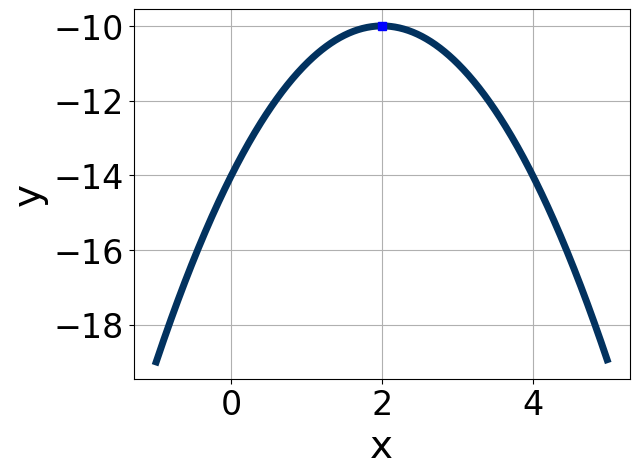
\includegraphics[width=0.5\textwidth]{../Figures/quadraticGraphToEquationB.png}
\end{center}
\begin{enumerate}[label=\Alph*.]
\item \( a \in [-1, 0], \hspace*{5mm} b \in [8, 9], \text{ and } \hspace*{5mm} c \in [-24, -23] \)
\item \( a \in [-1, 0], \hspace*{5mm} b \in [-8, -5], \text{ and } \hspace*{5mm} c \in [-24, -23] \)
\item \( a \in [0, 2], \hspace*{5mm} b \in [8, 9], \text{ and } \hspace*{5mm} c \in [8, 12] \)
\item \( a \in [0, 2], \hspace*{5mm} b \in [-8, -5], \text{ and } \hspace*{5mm} c \in [8, 12] \)
\item \( a \in [-1, 0], \hspace*{5mm} b \in [-8, -5], \text{ and } \hspace*{5mm} c \in [-10, -6] \)

\end{enumerate} }
\litem{
Graph the equation below.\[ f(x) = (x-3)^2 - 15 \]\begin{enumerate}[label=\Alph*.]
\begin{multicols}{2}\item 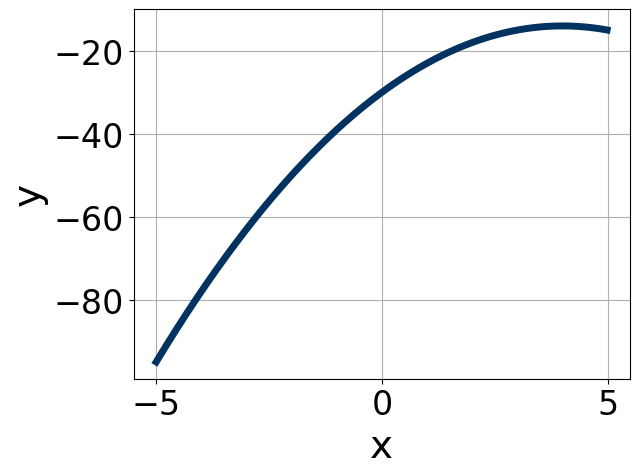
\includegraphics[width = 0.3\textwidth]{../Figures/quadraticEquationToGraphCopyAB.png}\item 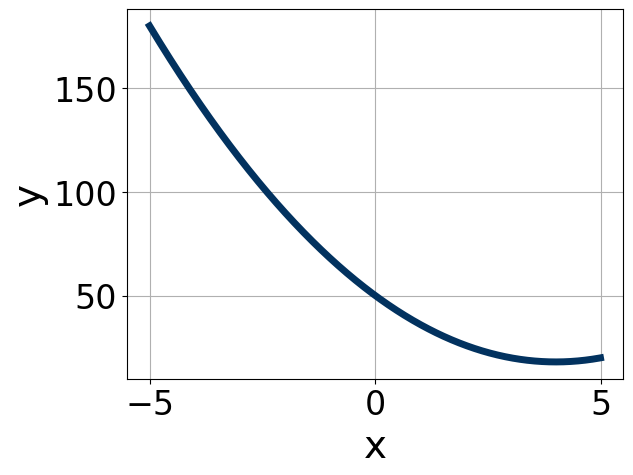
\includegraphics[width = 0.3\textwidth]{../Figures/quadraticEquationToGraphCopyBB.png}\item 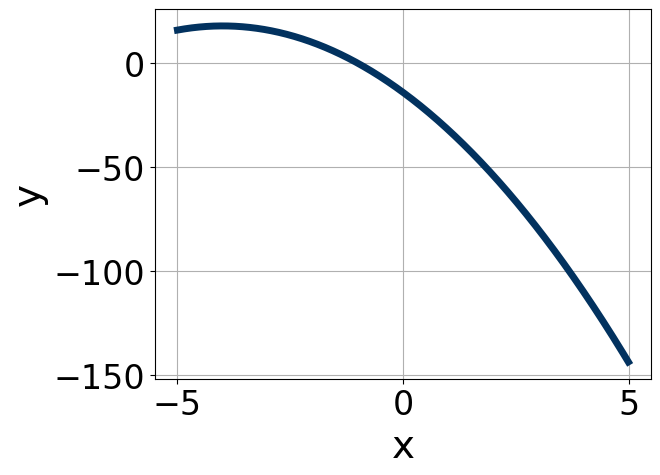
\includegraphics[width = 0.3\textwidth]{../Figures/quadraticEquationToGraphCopyCB.png}\item 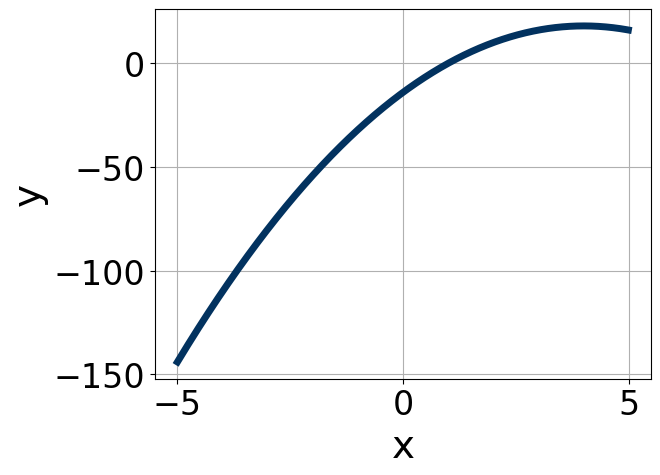
\includegraphics[width = 0.3\textwidth]{../Figures/quadraticEquationToGraphCopyDB.png}\end{multicols}\item None of the above.
\end{enumerate} }
\litem{
Write the equation of the graph presented below in the form $f(x)=ax^2+bx+c$, assuming  $a=1$ or $a=-1$. Then, choose the intervals that $a, b,$ and $c$ belong to.
\begin{center}
    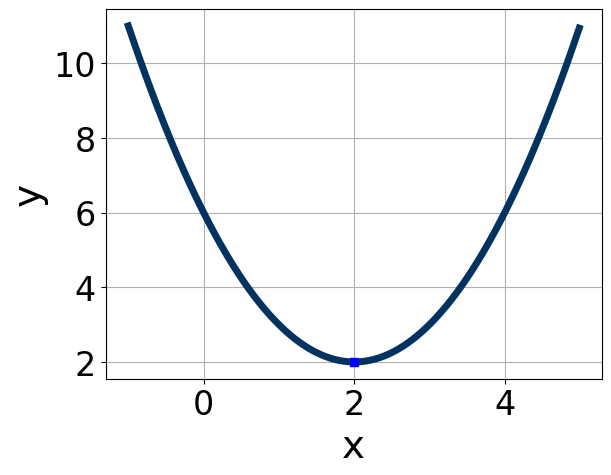
\includegraphics[width=0.5\textwidth]{../Figures/quadraticGraphToEquationCopyB.png}
\end{center}
\begin{enumerate}[label=\Alph*.]
\item \( a \in [-1.2, 0.1], \hspace*{5mm} b \in [-8, -7], \text{ and } \hspace*{5mm} c \in [-12, -8] \)
\item \( a \in [-1.2, 0.1], \hspace*{5mm} b \in [-8, -7], \text{ and } \hspace*{5mm} c \in [-20, -19] \)
\item \( a \in [0.8, 1.5], \hspace*{5mm} b \in [-8, -7], \text{ and } \hspace*{5mm} c \in [10, 15] \)
\item \( a \in [-1.2, 0.1], \hspace*{5mm} b \in [8, 10], \text{ and } \hspace*{5mm} c \in [-20, -19] \)
\item \( a \in [0.8, 1.5], \hspace*{5mm} b \in [8, 10], \text{ and } \hspace*{5mm} c \in [10, 15] \)

\end{enumerate} }
\litem{
Solve the quadratic equation below. Then, choose the intervals that the solutions belong to, with $x_1 \leq x_2$ (if they exist).\[ -14x^{2} -7 x + 9 = 0 \]\begin{enumerate}[label=\Alph*.]
\item \( x_1 \in [-23.92, -23.13] \text{ and } x_2 \in [21.7, 23.6] \)
\item \( x_1 \in [-0.62, -0.58] \text{ and } x_2 \in [0.6, 2.3] \)
\item \( x_1 \in [-8.52, -7.67] \text{ and } x_2 \in [13.5, 15.4] \)
\item \( x_1 \in [-1.24, -0.71] \text{ and } x_2 \in [0, 0.8] \)
\item \( \text{There are no Real solutions.} \)

\end{enumerate} }
\litem{
Factor the quadratic below. Then, choose the intervals that contain the constants in the form $(ax+b)(cx+d); b \leq d.$\[ 36x^{2} +53 x + 10 \]\begin{enumerate}[label=\Alph*.]
\item \( a \in [16.4, 18.5], \hspace*{5mm} b \in [-2, 5], \hspace*{5mm} c \in [1.22, 2.47], \text{ and } \hspace*{5mm} d \in [3, 11] \)
\item \( a \in [2, 6.3], \hspace*{5mm} b \in [-2, 5], \hspace*{5mm} c \in [10.79, 12.38], \text{ and } \hspace*{5mm} d \in [3, 11] \)
\item \( a \in [0.8, 2.1], \hspace*{5mm} b \in [8, 10], \hspace*{5mm} c \in [-0.82, 1.03], \text{ and } \hspace*{5mm} d \in [40, 47] \)
\item \( a \in [6.9, 10], \hspace*{5mm} b \in [-2, 5], \hspace*{5mm} c \in [3.28, 4.4], \text{ and } \hspace*{5mm} d \in [3, 11] \)
\item \( \text{None of the above.} \)

\end{enumerate} }
\litem{
Solve the quadratic equation below. Then, choose the intervals that the solutions $x_1$ and $x_2$ belong to, with $x_1 \leq x_2$.\[ 15x^{2} -38 x + 24 = 0 \]\begin{enumerate}[label=\Alph*.]
\item \( x_1 \in [0.66, 0.76] \text{ and } x_2 \in [2.28, 2.56] \)
\item \( x_1 \in [17.93, 18.08] \text{ and } x_2 \in [19.97, 20.17] \)
\item \( x_1 \in [1.15, 1.46] \text{ and } x_2 \in [1.21, 1.54] \)
\item \( x_1 \in [0.3, 0.44] \text{ and } x_2 \in [3.91, 4.31] \)
\item \( x_1 \in [0.44, 0.63] \text{ and } x_2 \in [2.45, 2.76] \)

\end{enumerate} }
\litem{
Factor the quadratic below. Then, choose the intervals that contain the constants in the form $(ax+b)(cx+d); b \leq d.$\[ 54x^{2} +33 x -10 \]\begin{enumerate}[label=\Alph*.]
\item \( a \in [7, 16], \hspace*{5mm} b \in [-2, 3], \hspace*{5mm} c \in [3.8, 7.8], \text{ and } \hspace*{5mm} d \in [4, 6] \)
\item \( a \in [20, 32], \hspace*{5mm} b \in [-2, 3], \hspace*{5mm} c \in [1.2, 3.8], \text{ and } \hspace*{5mm} d \in [4, 6] \)
\item \( a \in [-2, 2], \hspace*{5mm} b \in [-12, -10], \hspace*{5mm} c \in [-0.9, 1.6], \text{ and } \hspace*{5mm} d \in [39, 48] \)
\item \( a \in [2, 7], \hspace*{5mm} b \in [-2, 3], \hspace*{5mm} c \in [17.9, 20.8], \text{ and } \hspace*{5mm} d \in [4, 6] \)
\item \( \text{None of the above.} \)

\end{enumerate} }
\litem{
Graph the equation below.\[ f(x) = (x-1)^2 + 12 \]\begin{enumerate}[label=\Alph*.]
\begin{multicols}{2}\item 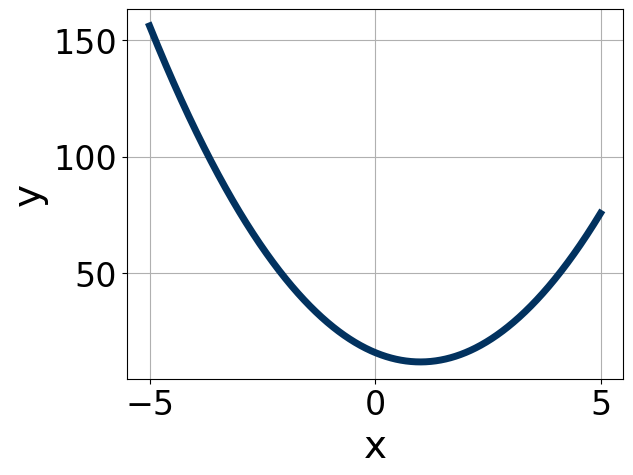
\includegraphics[width = 0.3\textwidth]{../Figures/quadraticEquationToGraphAB.png}\item 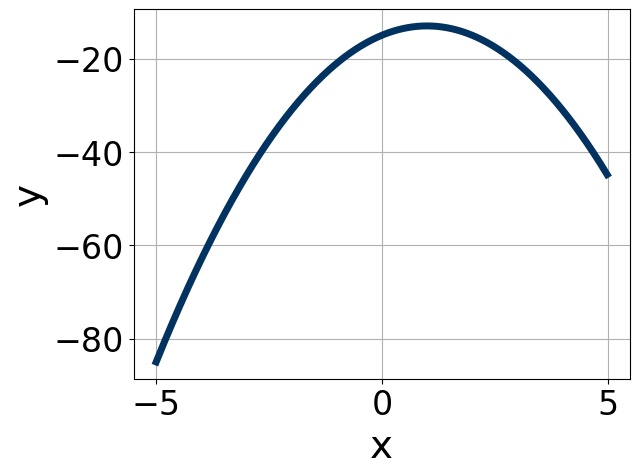
\includegraphics[width = 0.3\textwidth]{../Figures/quadraticEquationToGraphBB.png}\item 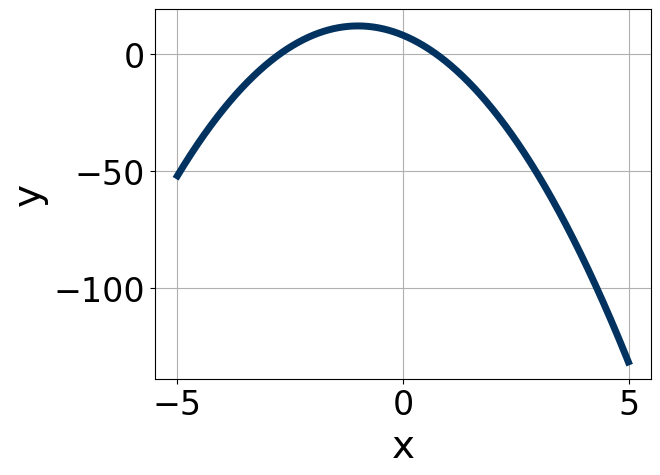
\includegraphics[width = 0.3\textwidth]{../Figures/quadraticEquationToGraphCB.png}\item 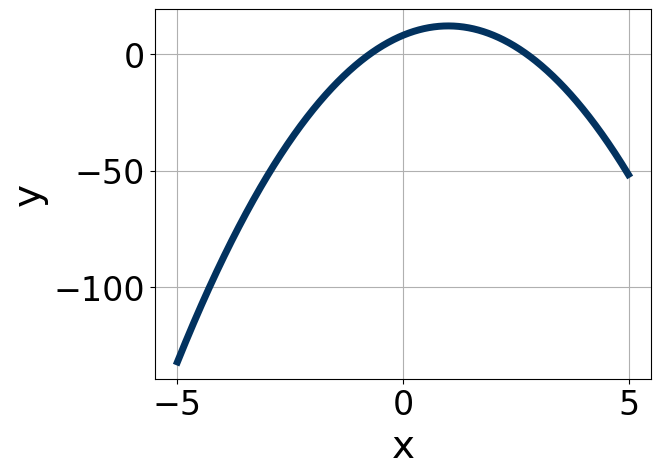
\includegraphics[width = 0.3\textwidth]{../Figures/quadraticEquationToGraphDB.png}\end{multicols}\item None of the above.
\end{enumerate} }
\end{enumerate}

\end{document}